
\section{Agents and Agent Based Modeling in Cyclus}\label{abm:abm}

\Cyclus has worked to formally move from a modeling paradigm that does not
differentiate between individual facilities, as has been the case historically
in FCS, to one that does. Modeling individual facilities in the NFC requires a
nuanced approach to determine facility behavior, because such behavior can
depend on intricate physical parameters of resources in the simulation as well
as complex social-behavioral models of facility interaction.

Agent-based models are defined primarily by two concepts: agents and the
simulation environment. Agents in Cyclus are designed to be able to incorporate
arbitrary complexity in both physical process models as well as behavioral
models. A three-tiered taxonomy has been developed to achieve this aim,
specializing agents as either Facilities, Institutions, or Regions. \S
\ref{abm:abm:tax} fleshes out a discussion of this design.

The simulation environment in Cyclus is defined by supply and demand. There is a
notion of supply and demand for facility capacity. For example, there can be a
demand for power production which drives the deployment of power producing
facilities. There is also a notion of supply and demand for resources. 

Sufficiently treating resource supply and demand is the primary argument for
implementing Cyclus as an ABM simulator. In the NFC, resource supply and demand
is a function of both resource quantity and quality, that is, the isotopic
composition of material resources. In the extreme in which a high level of
detail is required in the notion of resource quality, e.g. tracking an arbitrary
number of isotopes, adopting techniques that allow decision-making based on that
level of detail is desirable. Modeling the nuclear fuel cycle represents such a
level of detail. For example, even in the case of a once-through fuel cycle,
many reactors of the same type (e.g., PWRs), may require different resource
qualities (i.e., Uranium enrichment). As the complexity of a quality metric
increases, an aggregate approach becomes less desirable as it loses such detail
through aggregation. Furthermore, by dissasociating simulation logic from entity
logic, agents of arbitrary fidelity levels can be used in the same
simulation. For instance, a reactor agent that tracks a small subset of isotopes
can be used in tandem with a reactor agent that tracks a large set of isotopes.

In summary, the arbitrary levels of complexity that can be required for a
flexible NFC simulator suggests that ABM is a reasonable tool to use. The
remainder of this section describes how agents are provided agency in Cyclus and
specifically how agents interact with respect to supply and demand of facility
capacity. A proof-of-principle benchmark comparison to a systems dynamics
simulator is shown in \secref{abm:abm:proof}. Agent interaction with respect to
supply and demand of resources is more complicated and therefore treated
separately in \secref{abm:dre}.

\subsection{Agent Taxonomy}\label{abm:abm:tax}

The Cyclus kernel implements a basic \texttt{Agent} class that provides the
minimal interface for agents to be instantiated within a simulation. A
\texttt{Trader} interface provides a communication layer required for agents to be
included in the exchange of resources. Three useful derived classes are provided
to be used as basic abstractions of entities in the NFC. \texttt{Facility} agents
in Cyclus implement both interfaces, while \texttt{Institution} and \texttt{Region}
agents implement only the \texttt{Agent} interface.  A summary of the conceptual
placing of each archetype in a Cyclus simulation is provided below.

\subsubsection{Facilities}

Facilities in \Cyclus are either consumers or suppliers of commodities, and some
may be both. Supplier agents are provided agency by being able to communicate to
the market-resolution mechanism a variety of production capacity constraints in
second phase of the information gathering methodology. Consumer agents are
provided agency by being able to assign preferences among possible suppliers
based on the supplier's quality of product. Because this agency is encapsulated
for each agent, it is possible to define strategies that can be attached or
detached to the agents at run-time. Such strategies are an example of the
Strategy design pattern \cite{vlissides_design_1995}.

\subsubsection{Institutions}

Institutions in \Cyclus manage a set of facilities. Facility management is
nominally split into two main categories: the commissioning and decommissioning
of facilities and supply-demand association. The goal of including a notion of
institutions is to allow an increased level of detail when investigating
regional-specific scenarios. For example, a consumer facility may prefer to be
supplied by a supplier facility in its institution rather than one associated with
a different institution. Furthermore, there are international governmental
organizations, such as the IAEA, that have proposed managing large fuel cycle
facilities that service many countries in a given global region. A fuel bank is
an example of such a facility. Accordingly, institutions in \Cyclus are able to
augment the preferences of supplier-consumer pairs that have been established in
order to simulate a mutual preference to trade material within an
institution. Of course, situations arise in real life where an institution has
the capability to service its own facilities, but choose to use an outside
provider because of either cost or time constraints. Such a situation is allowed
in this framework as well. It is not clear how such a relationship should be
instantiated and to what degree institutions should be allowed to affect their
managed facilities' preferences. This issue lies squarely in the realm of
simulation design decisions, part of the \textit{art} of
simulation. Accordingly, through the course of research, the possible design
space will be analyzed in order to determine best practices for this type of
design.

\subsubsection{Regions}

Regions in \Cyclus provide the forcing function for simulations by requiring
that certain parameters be met, e.g., power capacity, fuel cycle service
capacity, etc. For example, in the case of nuclear power capacity, a region
knows that it needs additional reactors to be built, but leaves the building of
those reactors to the institutions that operate in the region. It is important
to note here that this abstraction allows for different deployment algorithms to
be tested and exchanged in the \Cyclus framework without necessitating changes
to the simulation engine, as is the case with other simulators described in
\secref{intro:fcs}.

Regions, like Institutions, are able to affect preferences between
supplier-consumer facility pairs in the market information gathering
process. The ability to perturb arc preferences between a given supplier and a
given consumer allows fuel cycle simulation developers to model relatively
complex interactions at a regional level such as tariffs and sanctions.

\subsection{Methods of Agency}\label{abm:abm:agent}

Agency is provided in two primary modes: determining facility deployment and
informing resource exchange mechanisms. 

Facility deployment involves some combination of an \texttt{Institution} agent, a
\texttt{Facility} agent, and a \texttt{Region} agent. \texttt{Institution} agents
represent a simulation entity abstraction that can deploy \texttt{Facility}
agents. \texttt{Region} agents represent a simulation entity abstraction that have
a demand for certain commodities that \texttt{Facility} agents provide, for
example, reactor-like \texttt{Facility} agents provide electrical power.

\texttt{Facility} agents are further provided agency by informing market
mechanisms of the supply and demand of resource quantity and quality. Cyclus
initially used a simple interface and algorithm for determining resource
transactions. Individual markets were defined as agents themselves much like
\texttt{Facility}, \texttt{Institution}, and \texttt{Region} agents. Many limitations
were identified at the time, however, and the market-as-agent approach was
eventually abandoned. An enumeration of the observed limitations is described
further in \secref{abm:abm:limits}.

The primary source of agency is provided to \texttt{Facility} agents through the
\texttt{Trader} interface in order to negotiate the quantity and quality of
potential resource transactions. \texttt{Region}, \texttt{Institution}, and
\texttt{Facility} agents are then provided agency in the negotiation of
preferences of potential transactions, where preference is a proxy for price.

\subsection{Proof of Principle}\label{abm:abm:proof}

Agents were developed to show an initial proof of principle that fuel cycle
simulation can be implemented using an agent-based modeling methodology. By
definition, dynamic simulators model the deployment of facilities and measure
the flow of resources between facilities in the system over time. In the extreme
case of unconstrained supply and no competition for resources, resource exchange
decisions can be made arbitrarily. In such cases, therefore, only facility
deployment agency is required. An initial benchmark case was performed to
confirm expected deployment behavior and basic resource routing.

\subsubsection{Benchmark Cases}

The INPRO Business As Usual (BAU) benchmark \cite{_international_2009} for the
once-through fuel cycle was chosen for three reasons. First, it was the simplest
benchmark that demonstrated deployment behavior. Second, no supply or demand
constraints were present, so a basic supply-demand framework would
suffice. Finally, results from another fuel cycle simulation texttt, specifically
VISION \cite{vision2009}, was available for comparison. The INPRO BAU benchmark
identified two cases, high electricity demand and moderate electricity demand,
as shown in Fig. \ref{fig:inpro-demand}. Both cases require that demand met by a
composition of 94\% Light Water Reactors (LWRs) and 6\% Heavy Water Reactors
(HWRs). LWRs are fueled with 4\% by weight UO$_2$ while HWRs use natural Uranium
fuel.

\begin{figure}
  \begin{center}
    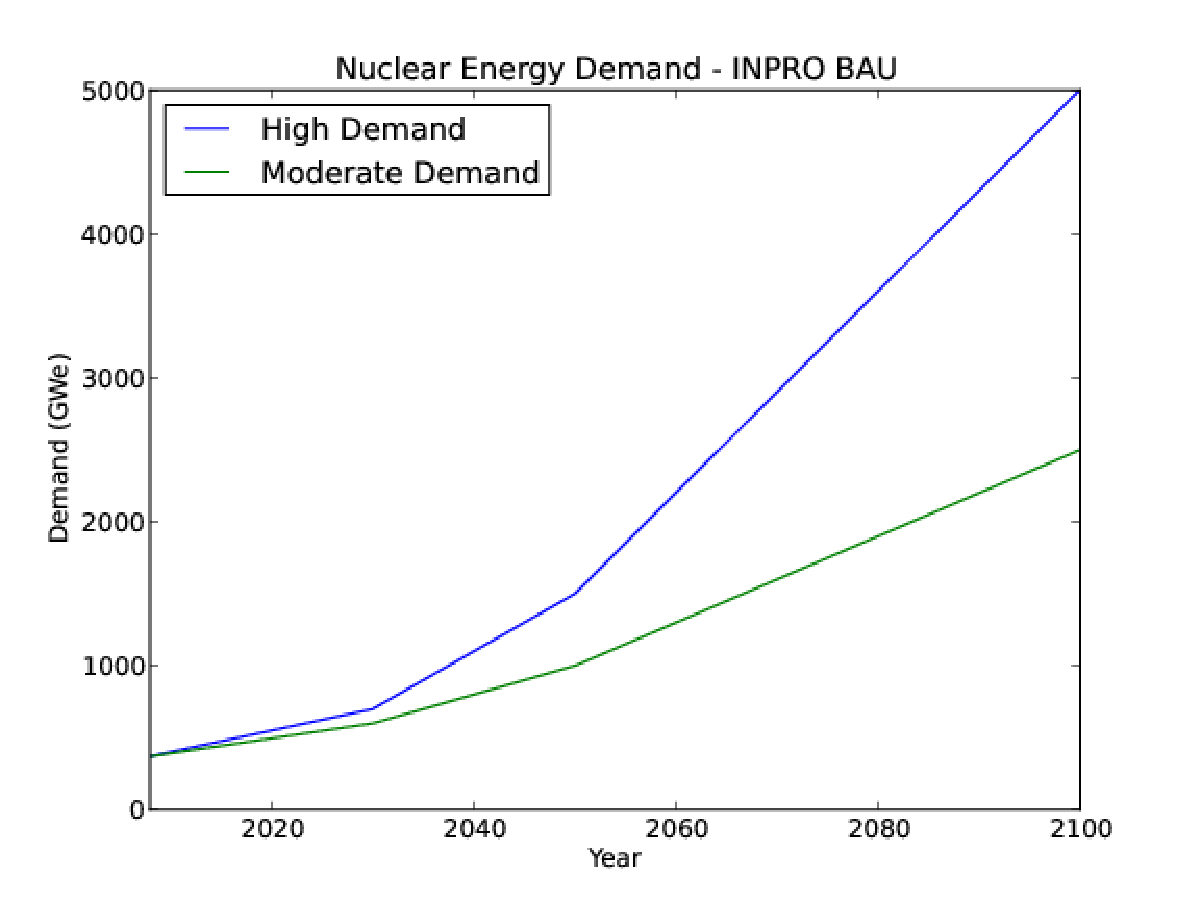
\includegraphics[height=8cm]{inpro-demand.pdf}
    \caption{The energy demand specification for the INPRO BAU scenarios.}
    \label{fig:inpro-demand}
  \end{center}  
\end{figure}

The goal of this proof-of-principle study was to showcase the capability for a
developer to generate the required Facility, Institution, and Region archetypes,
and that such archetypes could be deployed in the Cyclus simulation framework
and generate satisfactory results. Comparison metrics are based on similar
metrics used in the origin INPRO benchmarking exercise, including deployment
patterns, natural uranium consumed, and used fuel produced by all reactors.

\subsubsection{Agent Archetypes Developed}

Each implemented agent is available in the Cycamore repository \cite{cycamore2013}.

\paragraph{GrowthRegion}

The \texttt{GrowthRegion} is a Region archetype developed to assist in
facility deployment logic. The \texttt{GrowthRegion} takes as input a listing of
commodities for which it has a demand. For example, the \texttt{GrowthRegion}
agents in this benchmark demand electrical power. The demand curves for
commodities is defined by symbolic functions. Currently, linear functions,
exponential functions, and piece-wise combinations of both are supported.

At any time step in which there exists a demand gap, i.e., there exists more
demand than supply, a build decision is made. This decision is modeled as the
following minimum cost facility deployment integer program:
%%%
\begin{subequations} \label{eqs:growth}
\begin{equation} \label{eq:optBuildObj}
\begin{aligned}
& \min_{n}
& & \sum_{i \in I} c_i * n_i
\end{aligned}
\end{equation}
\begin{equation} \label{eq:optBuildConst}
\begin{aligned}
& \text{s.t.}
& & \sum_{i \in I} \phi_i * n_i  \ge \Phi
\end{aligned}
\end{equation}
\begin{equation} \label{eq:optBuildBounds}
\begin{aligned}
& n_i \in [0,\infty) & \forall \:\: i \in I &
\end{aligned}
\end{equation}
\begin{equation} \label{eq:optBuildInt}
\begin{aligned}
& n_i \:\:\: integer & \forall \:\: i \in I &
\end{aligned}
\end{equation}
where $\Phi$ is the unmet demand, $I$ is the set of facilities capable of 
meeting the demand, and, for each facility in $I$, $c_i$ is the cost of building, 
and $\phi_i$ is the nameplate capacity.  Finally, $n_i$ is the optimized number of
facilities to build of type $i$.
\end{subequations}
%%%

\paragraph{ManagerInst}

The \texttt{ManagerInst} is an Institution archetype also developed to assist
in facility deployment. While the \texttt{GrowthRegion} places a build order, the
\texttt{ManagerInst} fulfills the order. Further, the \texttt{ManagerInst}
determines the set of facilities, $I$, shown in in Eqn. \ref{eqs:growth}, which
can be built. Note that the set $I$ can change over time. Once a deployment
decision is made, the \texttt{GrowthRegion} makes a facility deployment request of
the \texttt{ManagerInst} which then deploys the chosen facility.

\paragraph{BatchReactor}

While a reactor model existed prior to this work, it did not provide the
functionality to interchange \textit{batches} of fuel, as required by the INPRO
benchmark. A batch of fuel is a fraction of a full reactor core that is
extracted and replaced when a reactor is refueled. In general, LWRs replace
between a third and a quarter of their assemblies during refueling based on the
fuel management scheme used.

The \texttt{BatchReactor} used in this work had configurable properties as
displayed in Table \ref{tbl:batchrxtr}. The values used based on the defined
INPRO benchmark are described in Table \ref{tbl:inprorxtr}.

\begin{table}[h]
\centering
\begin{tabular}{cc}
Parameter      & Description                     \\ \hline
Process Time   & Active fuel time in the reactor                        \\
Refuel Time    & Time to refuel the reactor                              \\
N Batches      & Number of batches in the reactor                         \\
Batch Size     & Quantity of a batch                                 \\
Power Capacity & Nameplate Capacity for Power                          \\
Power Cost     & Cost to build a new reactor      \\ \hline
\end{tabular}
\caption{Configurable input for the \texttt{BatchReactor} archetype.}
\label{tbl:batchrxtr}
\end{table}

\begin{table}[h]
\centering
\begin{threeparttable}
\begin{tabular}{ccc}
Parameter      & LWR Value & HWR Value               \\ \hline
Process Time   & 10         & 10                       \\
Refuel Time    & 2          & 2                        \\
N Batches      & 4          & 4                        \\
Batch Size     & 7.87E4     & 1.39e5                   \\
Power Capacity & 1000       & 600                      \\
Power Cost     & 1000*      & 600* \\ \hline
\end{tabular}
\begin{tablenotes}
  \small
  \item (*) Note that the Cost used is arbitrary and set equal to the
  capacity so that a minimum capacity is built per Eqn. \ref{eqs:growth}.
\end{tablenotes}
\end{threeparttable}
\caption{Configurable input values for reactors used in the INPRO once-through benchmark.}
\label{tbl:inprorxtr}
\end{table}

\paragraph{EnrichmentFacility}

The \texttt{EnrichmentFacility} archetype was developed to provide
enrichment-related output for the simulation, namely the amount of separative
work units (SWU) and natural uranium used during a given time step. For the
INPRO cases, it can be defined quite simply using the values shown in Table
\ref{tbl:inproenr}. The feed assay and product assay, both required for
determining output metrics, are defined by the isotopic compositions of
resource input, i.e., natural uranium, and resource output, i.e., the isotopic
composition of requested fuel.

\begin{table}[h]
\centering
\begin{tabular}{ccc}
Parameter    & Description                      & Values          \\ \hline
Input Recipe & A description of input isotopics & Natural Uranium \\
Tails Assay  & The U-235 assay of tails.        & 0.003          
\end{tabular}
\caption{Configurable input values for the \texttt{EnrichmentFacility} used in the
  INPRO once-through benchmark.}
\label{tbl:inproenr}
\end{table}

\subsubsection{Results}

% c/Cref is cleveref

In aggregate, Cyclus performed well relative to the other benchmark
texttts. Fig. \ref{fig:rxtrs_low} shows the reactor deployment curves for each
simulator for the moderate growth scenario while Fig. \ref{fig:rxtrs_high} shows
reactor deployment for the high scenario. The slight differences are attributed
to VISION's look-ahead functionality which builds the required facilities one
time step after they are needed, whereas Cyclus builds facilities on the
timestep in which they are needed. One can observe that a simple one timestep
translation will result in identical output.

Cumulative natural uranium utilization curves for the moderate and high cases
are shown in \Cref{fig:nat_u_low,fig:nat_u_high}, and cumulative used fuel
inventory curves are shown in
\Cref{fig:used_fuel_low,fig:used_fuel_high}. Slight discrepancies are noted
between Cyclus and VISION. These discrepancies are attributed to the
implementation of core batch recycling in each of the respective texttts. The
differences between Cyclus and VISION are magnified because the curves show
cumulative metrics. In other words, results at time $t_1$ are added the results
at time $t_2$ and so on. Therefore, a series of small discrepancies appears to
be compounded by using this metric. It is not the metric of choice for general
comparisons, but has been used because it was the metric of choice of the
benchmark exercise. It is not immediately obvious why there is a greater
discrepancy regarding output fuel quantities than natural uranium
utilization. Further benchmarking exercises with support from a VISION developer
would be required to fully investigate the issue.

\begin{figure}
  \begin{center}
    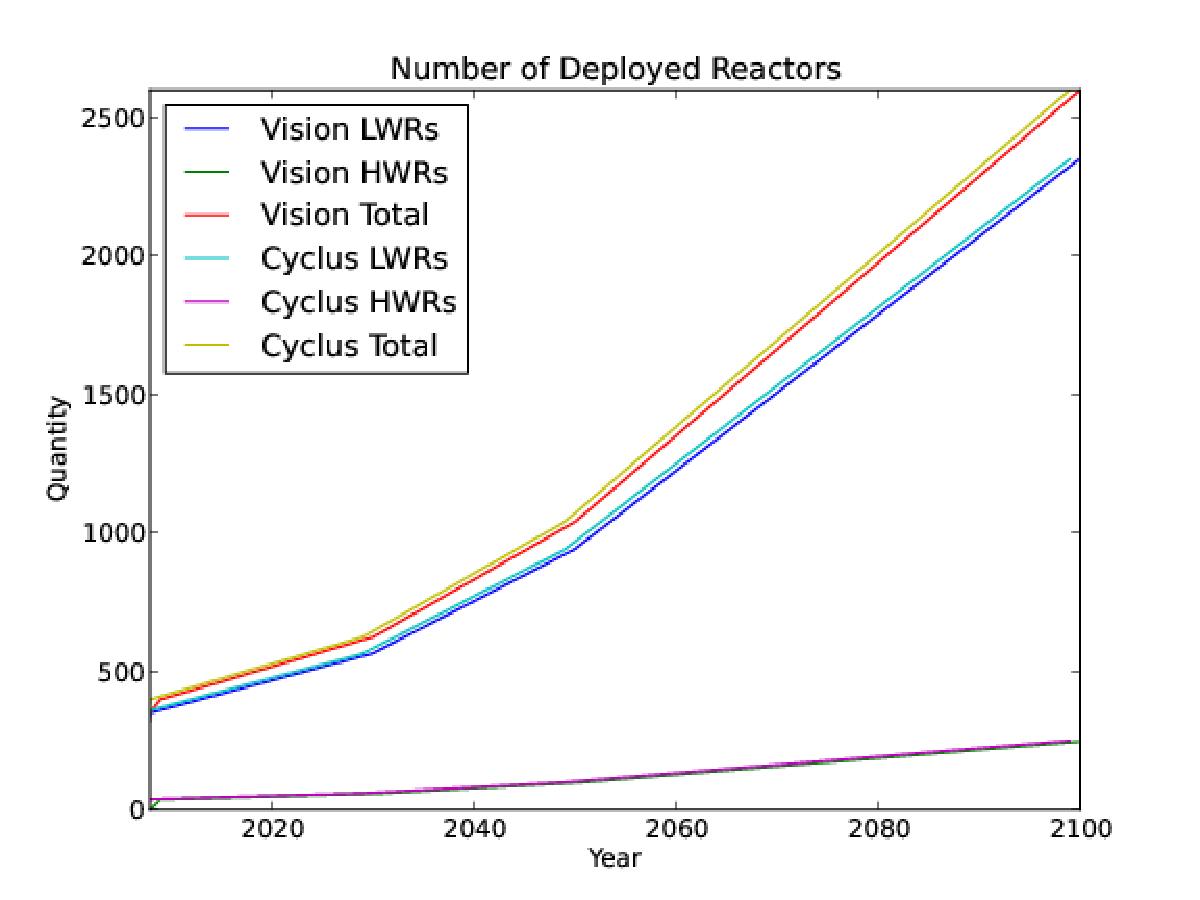
\includegraphics[height=8cm]{rxtrs_low.pdf}
    \caption{The reactor deployment schedule by reactor type for the moderate demand scenario.}
    \label{fig:rxtrs_low}
  \end{center}  
\end{figure}

\begin{figure}
  \begin{center}
    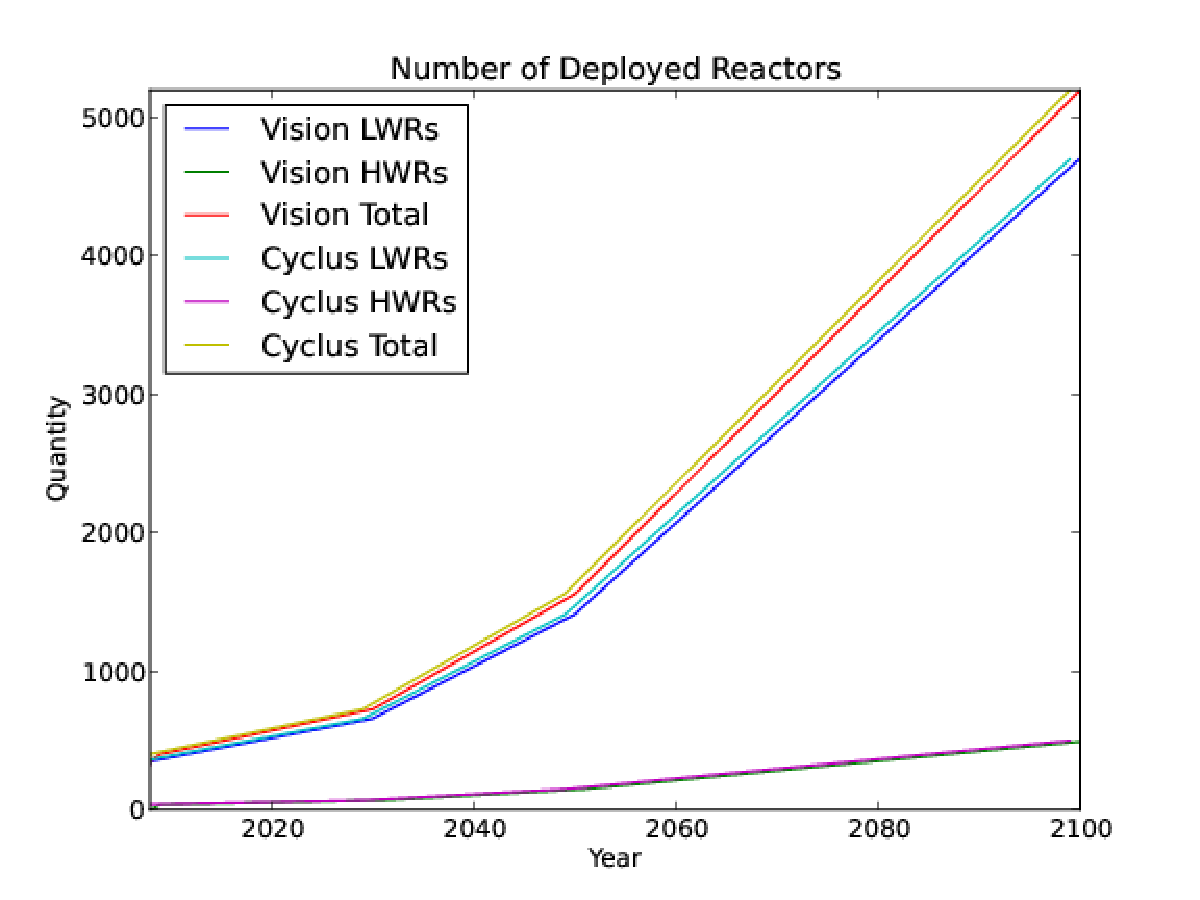
\includegraphics[height=8cm]{rxtrs_high.pdf}
    \caption{The reactor deployment schedule by reactor type for the high demand scenario.}
    \label{fig:rxtrs_high}
  \end{center}  
\end{figure}

\begin{figure}
\begin{center}
  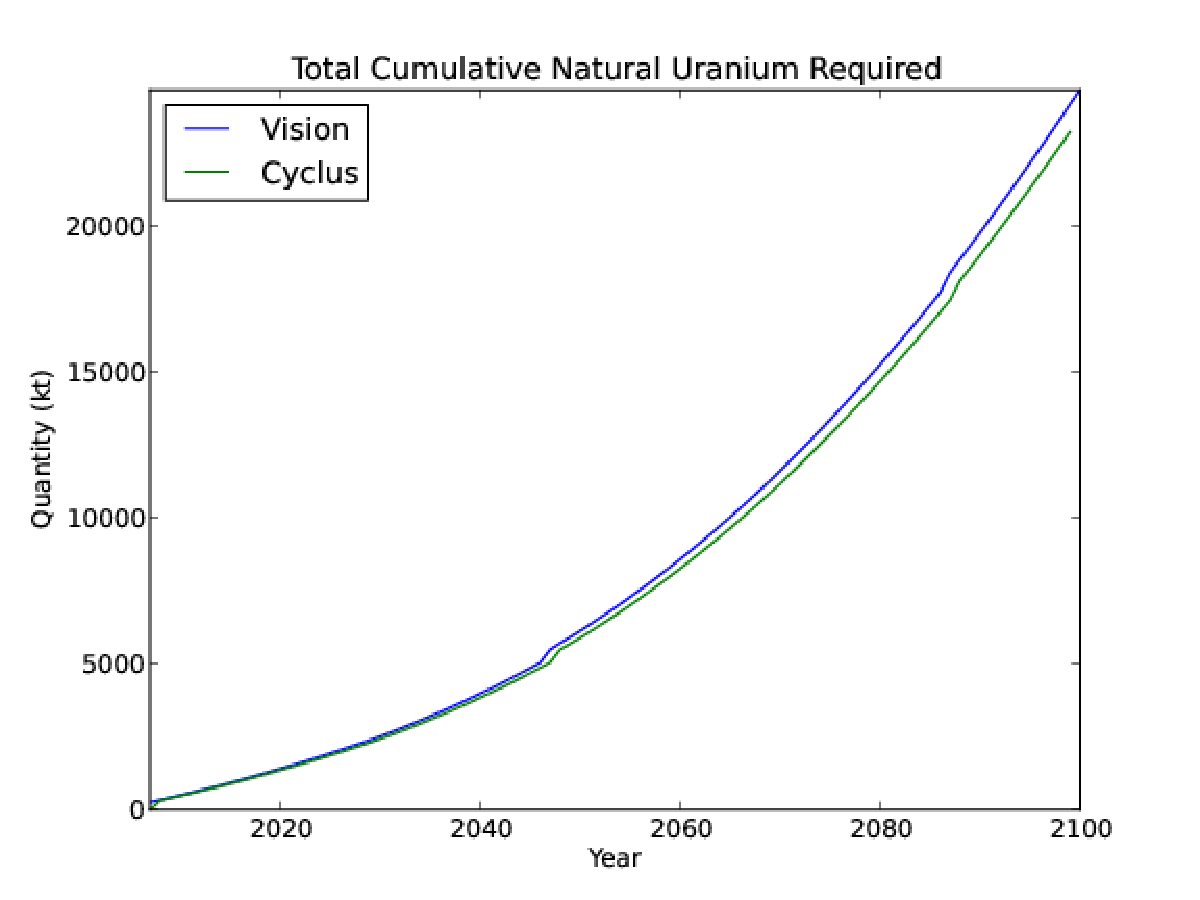
\includegraphics[height=8cm]{nat_u_low.pdf}
  \caption{The total natural uranium used for the moderate demand scenario.}
  \label{fig:nat_u_low}
\end{center}  
\end{figure}

\begin{figure}
\begin{center}
  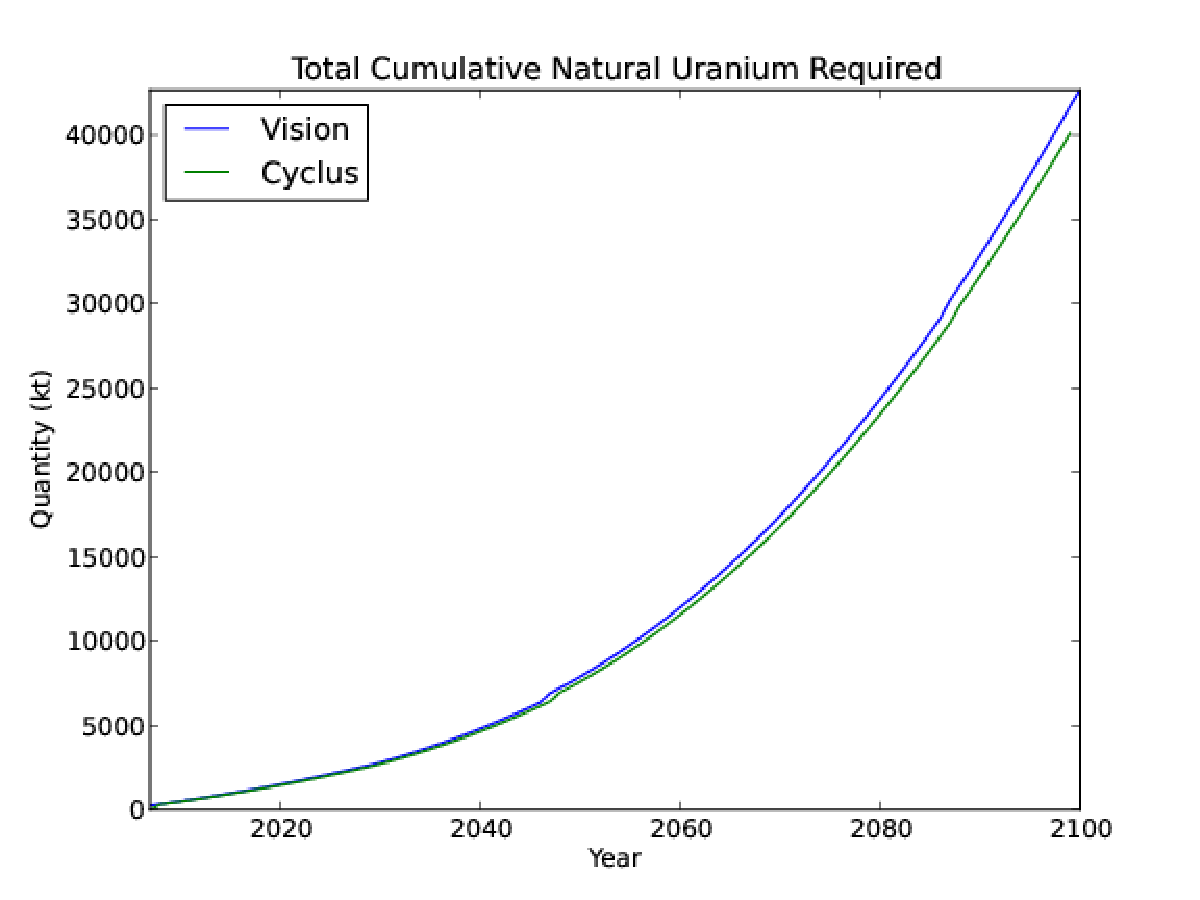
\includegraphics[height=8cm]{nat_u_high.pdf}
  \caption{The total natural uranium used for the high demand scenario.}
  \label{fig:nat_u_high}
\end{center}  
\end{figure}

\begin{figure}
  \begin{center}
    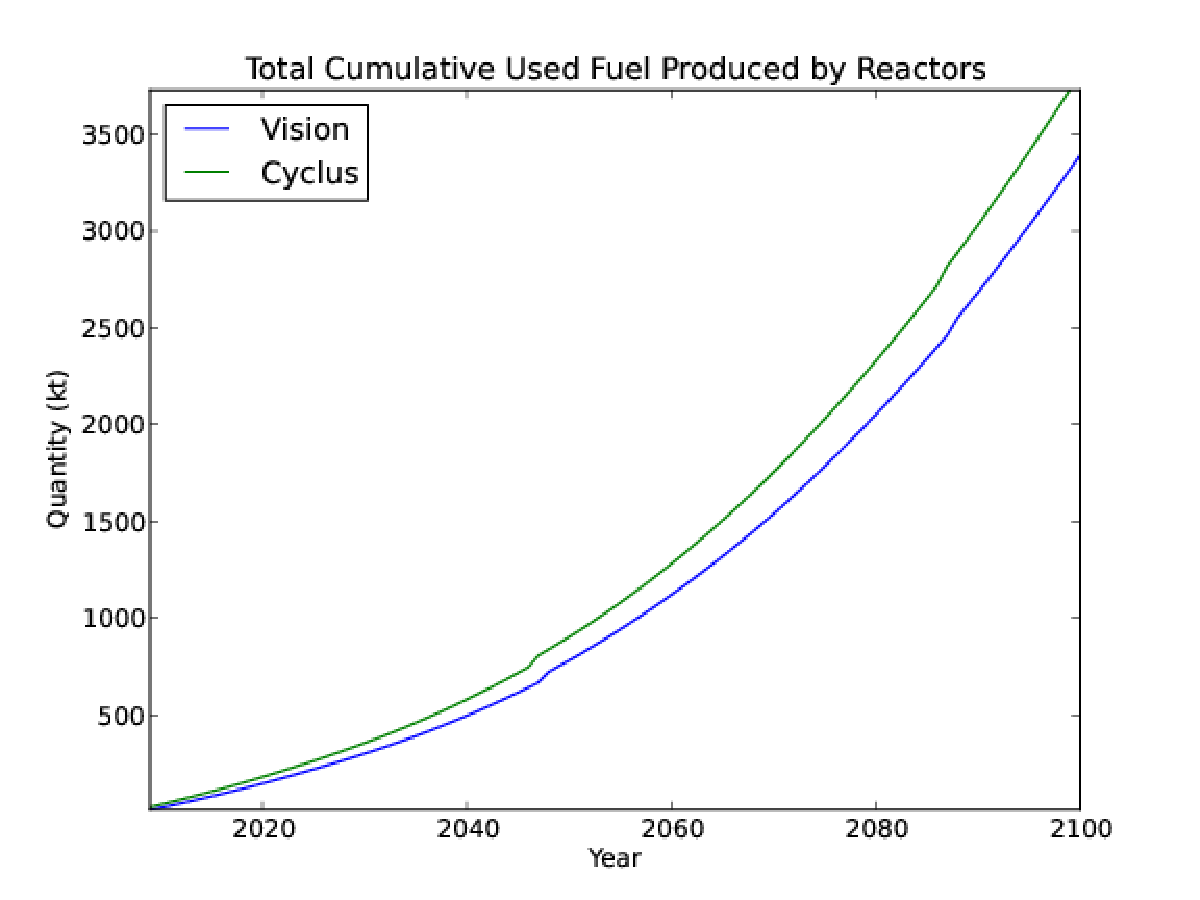
\includegraphics[height=8cm]{used_fuel_low.pdf}
    \caption{The amount of used fuel produced for the moderate demand scenario.}
    \label{fig:used_fuel_low}
  \end{center}  
\end{figure}

\begin{figure}
  \begin{center}
    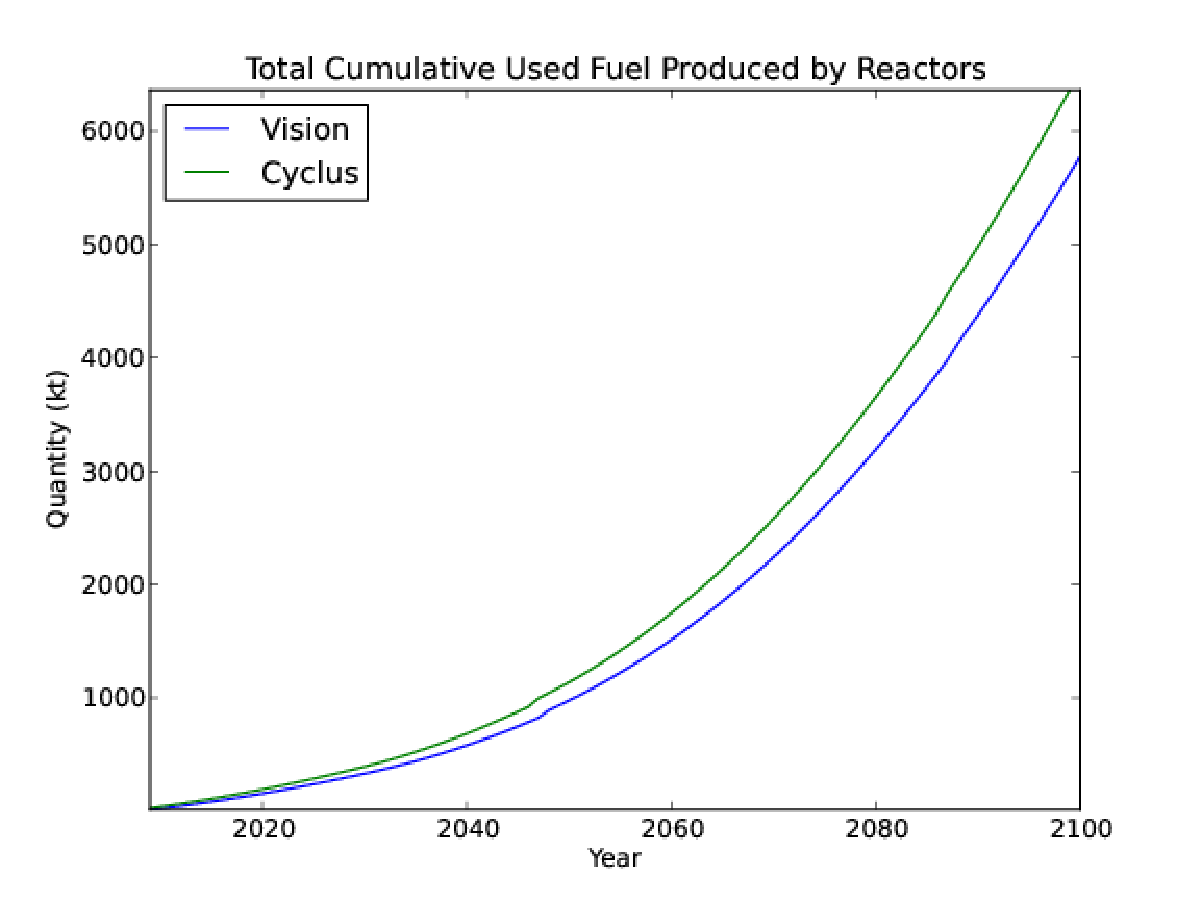
\includegraphics[height=8cm]{used_fuel_high.pdf}
    \caption{The amount of used fuel produced for the high demand scenario.}
    \label{fig:used_fuel_high}
  \end{center}  
\end{figure}

\subsection{Multiple Market Limitations}\label{abm:abm:limits}

The proof of principle benchmark described in \secref{abm:abm:proof} utilized
the agency provided for facility deployment rather than the agency provided for
both deployment and resource exchange. In general informing resource exchange
regarding quantity and quality of resources as well as socioeconomic effects is
a hard problem.

Cyclus was originally designed to use an additional agent archetype called a
\texttt{Market}. \texttt{Market}s were envisioned to represent markets for
specific commodities. For example, the simulation described in \S
\ref{abm:abm:proof} used three commodity markets: natural uranium, enriched
uranium fuel, and used fuel. This approach is valid in the absence
agent-specified supply or demand constraints and competition for resources in
multiple markets (e.g., for fungible resources). However, the inclusion of
either of these features requires a much more involved process.

If supply or demand constraints are to be modeled, each
associated \texttt{Market} agent must have both a corresponding communication
interface and an implementation that accounts for such constraints. While
quantity constraints are not unreasonable to implement and support, quality
constraints are much more difficult. Furthermore, communicating such constraints
is difficult. Whereas the \texttt{Market} agent can implement a solver algorithm,
constraints are more naturally defined by the trader interacting with the
\texttt{Market} agent. For example, consider the enriched uranium market used in
\secref{abm:abm:proof}. While the simulation used an agent abstraction for an
enrichment facility and fuel fabrication plant, another simulation may wish to
model facilities that downblend HEU, rather than enrich LEU. Such a process will
have different constraints. Importantly, those constraints are a function of the
\texttt{Facility} archetype, not of a \texttt{Market} archetype.

Assuming that supply or demand is constrained by either resource quantity or
quality, competition for the resource in question can arise.  When competition
for resources exist, there must be some mechanism that determines which
transactions are to be executed, i.e., which agents should trade which
resources. Determining supply and demand under competition is a well studied
problem with many possible formulations and solution frameworks.

Fungibility is the property of a good or commodity to be \textit{capable of
  being substituted in place of one another} \cite{MerriamWebster2014}. For
example, a light water reactor generates power by fissioning nuclei in the
thermal energy spectrum. Whether those nuclei are \nucl{239}{Pu}, \nucl{235}{U},
or \nucl{233}{U} makes little difference from a power generation perspective. In
other words, those nuclei are \textit{fungible} for light water reactors, given
some safety and cycle length considerations. A similar issue arises from a
supplier's perspective. Consider a MOX fuel supplier and two requesters: a fast
reactor and a thermal reactor. Given the isotopic makeup of Plutonium in the MOX
fuel, the supplier's fuel could be potentially be used in either reactor
type. Again, Plutonium in this example is a fungible resource. Importantly, the
notion of fungibility in a NFC context can refer to both individual isotopes,
collections of isotopes, or complete fuel forms. Accordingly, a facility may
demand multiple fungible commodities, which must be accounted for by a given
market clearing mechanism.

The one-market-per-commodity approach does not treat competition, constrained
supply and demand, and fungibility particularly well. Constraints are handled
poorly because constraints are best determined by the supplying and demanding
agents rather than the market. Separated markets must, of course, be solved
separately. Therefore, competition and fungibility are treated poorly, because
information involving multiple commodities is not taken into account during the
solution of a single market. Accordingly, a solution framework and methodology
that incorporates agent querying of supply, demand, and constraints and resolves
markets in parallel is required to properly treat resource exchange in the
nuclear fuel cycle.
